\documentclass{article}
\usepackage[utf8]{inputenc}
\usepackage[T1]{fontenc}
\usepackage{graphicx}        
\usepackage{caption}
\usepackage{booktabs}         
\usepackage{amsmath,amssymb}  
\usepackage{parskip} 
\usepackage{url} 
\usepackage{float}
\usepackage{array}
\usepackage{hyperref}

\usepackage{geometry}
\geometry{total = {8.5in,11in}, margin=1in}


\title{\textbf{Final project}}
\author{Mengying Xia}
\date{August 21 2025}

\begin{document}
\maketitle


\section{Introduction}

The abhydrolase domain containing 5, lysophosphatidic acid acyltransferase (ABHD5), is a gene located in 3p21.33, \cite{ref1} that is ubiquitously expressed in adipose tissue, bone marrow, and various other tissues. \cite{ref2}. ABHD5 is the causative gene of Chanarin–Dorfman syndrome, marked by accumulation of systemic triacylglycerol and altered skin barrier.\cite{ref3} The encoded protein consists of eight central beta strands, flanked by two and four alpha helices on each side, respectively. ABHD5 is a key regulator of lipid and energy homeostasis. Lacking intrinsic hydrolase activity, ABHD5 acts as a coactivator of enzymes of the PNPLA family involved in the metabolism of triacylglycerol, glycerophospholipid, sphingolipid and retinyl ester and interacts with perilipins and fatty acid binding proteins. \cite{ref4} Plasma and leukocyte samples from hospitalized patients with and without COVID-19 across severities were profiled. More than 17,000 transcripts, proteins, metabolites, and lipids were quantified, integrated with clinical data into a curated database, and 219 molecular features were identified as significantly associated with COVID-19 status and severity. \cite{ref5}

\section{Methods}
\subsection{Data Source}
All analyses in this study were conducted using publicly available datasets from the Gene Expression Omnibus under accession GSE157103. \cite{ref5} Data was collected from a large-scale multi-omic analysis of COVID-19 severity. 125 samples were included in the final analysis, with 51 women and 74 men, 100 with COVID-19 and 25 without COVID-19.

\subsection{R Version and Packages}
R version 4.5.1 was used for data analysis. The R packages knitr \cite{ref6} and dplyr \cite{ref7}  were used for data processing; kableExtra \cite{ref8} and table1 \cite{ref9} for tabular presentation of variable characteristics; and ggplot2 \cite{ref10}, pheatmap \cite{ref11}, and hexbin \cite{ref12} for data visualization.
\subsection{Clustering Algorithm}
Euclidean distance is used to identify how similar different samples. The algorithm for Euclidean distance is:
$$  d\left( p,q\right)   = \sqrt {\sum _{i=1}^{n}  \left( q_{i}-p_{i}\right)^2 }  $$


\section{Results}
\subsection{Table 1}


\begin{table}[H]
\centering
\caption{Baseline characteristics stratified by COVID status}
\label{tab:baseline}
\begin{tabular}{@{}p{6.2cm} >{\centering\arraybackslash}p{5cm} >{\centering\arraybackslash}p{5cm}@{}}
\toprule
Characteristic & COVID-19 (N = 100, 80.0\%) & Non-COVID-19 (N = 25, 20.0\%) \\
\midrule
\textbf{Sex}, n(\%) & & \\
\quad Female & 38 (38.0\%) & 13 (52.0\%)  \\
\quad Male   & 62 (62.0\%) & 12 (48.0\%) \\
\addlinespace
\textbf{ICU status}, n(\%)& &  \\
\quad Yes & 50 (50.0\%) & 15 (60.0\%) \\
\quad No  & 50 (50.0\%) & 10 (40.0\%) \\
\addlinespace
\textbf{Charlson score}, Median [IQR] & 3.0 [1.0, 5.0] & 4.0 [2.0, 6.0] \\
\addlinespace
\textbf{Ferritin (ng/ml)}, Median [IQR]& 652.0 [307.5, 1179.0] & 142.0 [83.5, 325.5] \\
\quad Missing & 6 (6.0\%) & 9 (36.0\%)\\
\addlinespace
\textbf{Procalcitonin (ng/ml)}, Median [IQR] & 0.6 [0.2, 1.8] & 0.4 [0.3, 0.7] \\
\quad Missing & 13 (13.0\%) & 10 (40.0\%) \\
\bottomrule
\end{tabular}
\end{table}

\subsection{Figure 1. Histogram}
\begin{figure}[H]
\centering
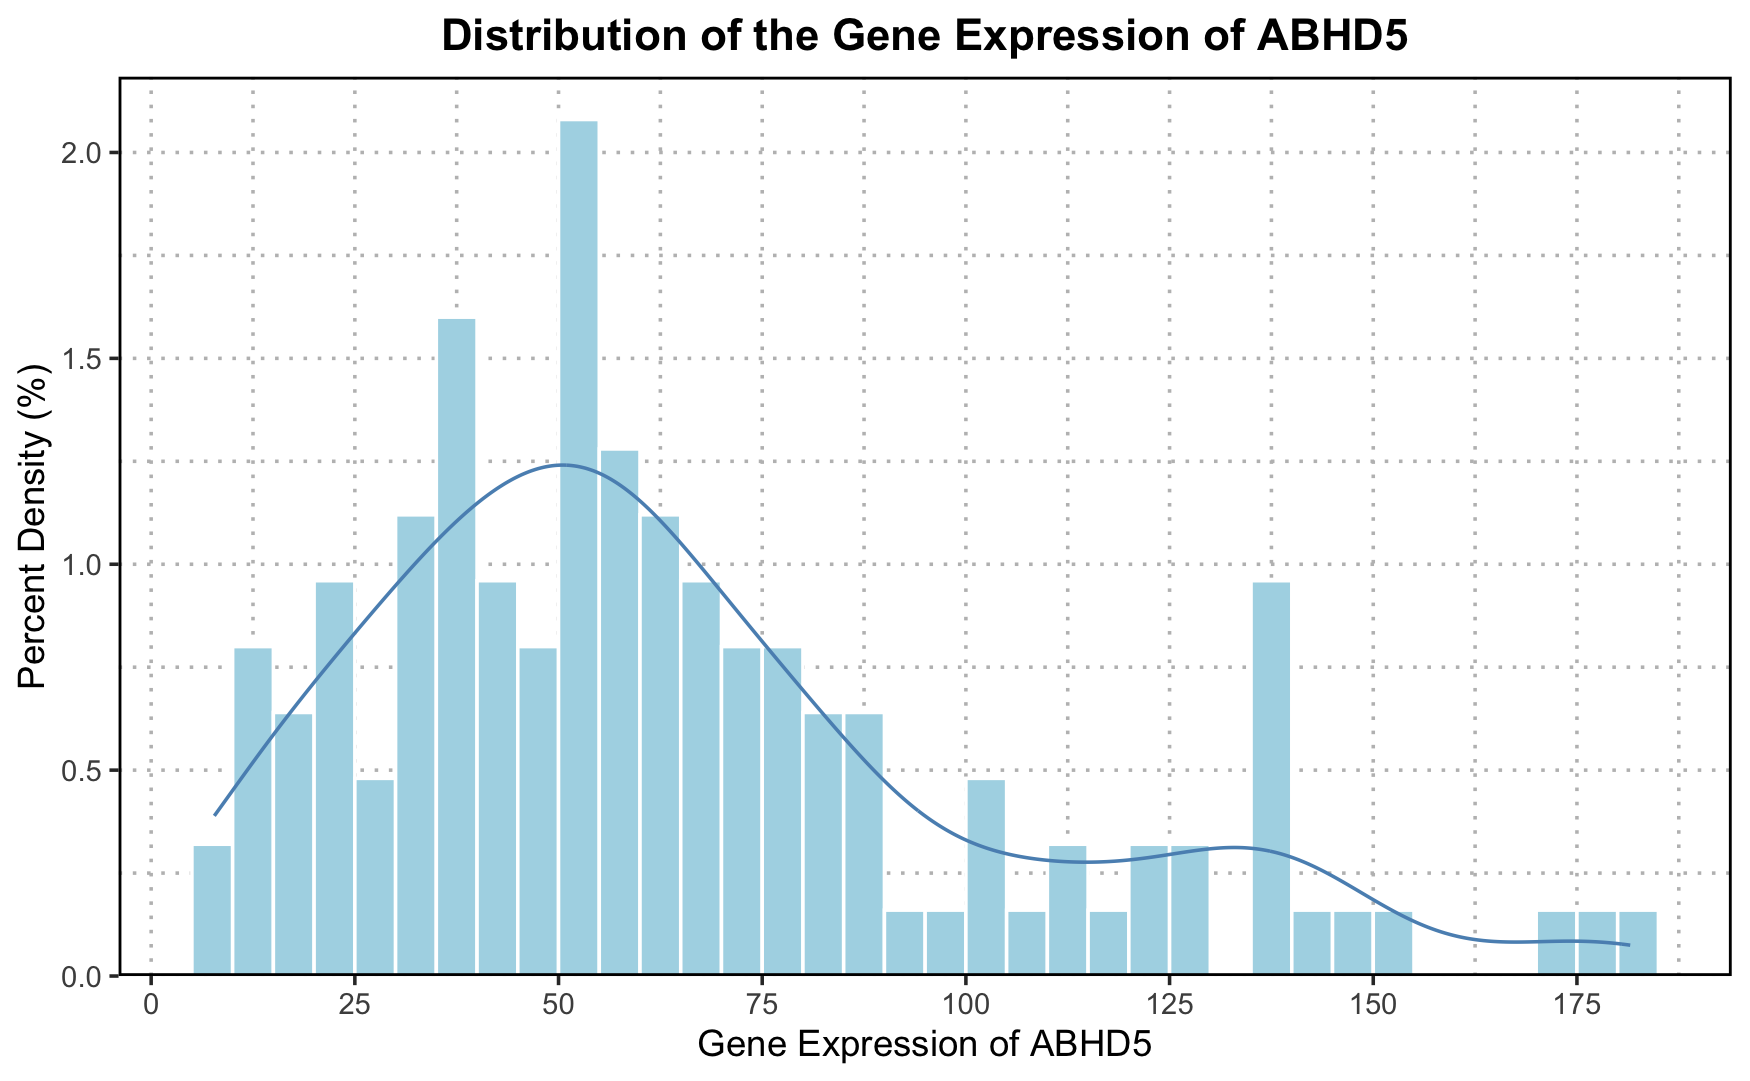
\includegraphics[width=1\linewidth]{Histogram.png}
\label{fig:histogram}
\end{figure}

The distribution of ABHD5 expression is right-skewed, with the peak near an expression value of about 50.

\subsection{Figure 2. Scatterplot}
\begin{figure}[H]
    \centering
    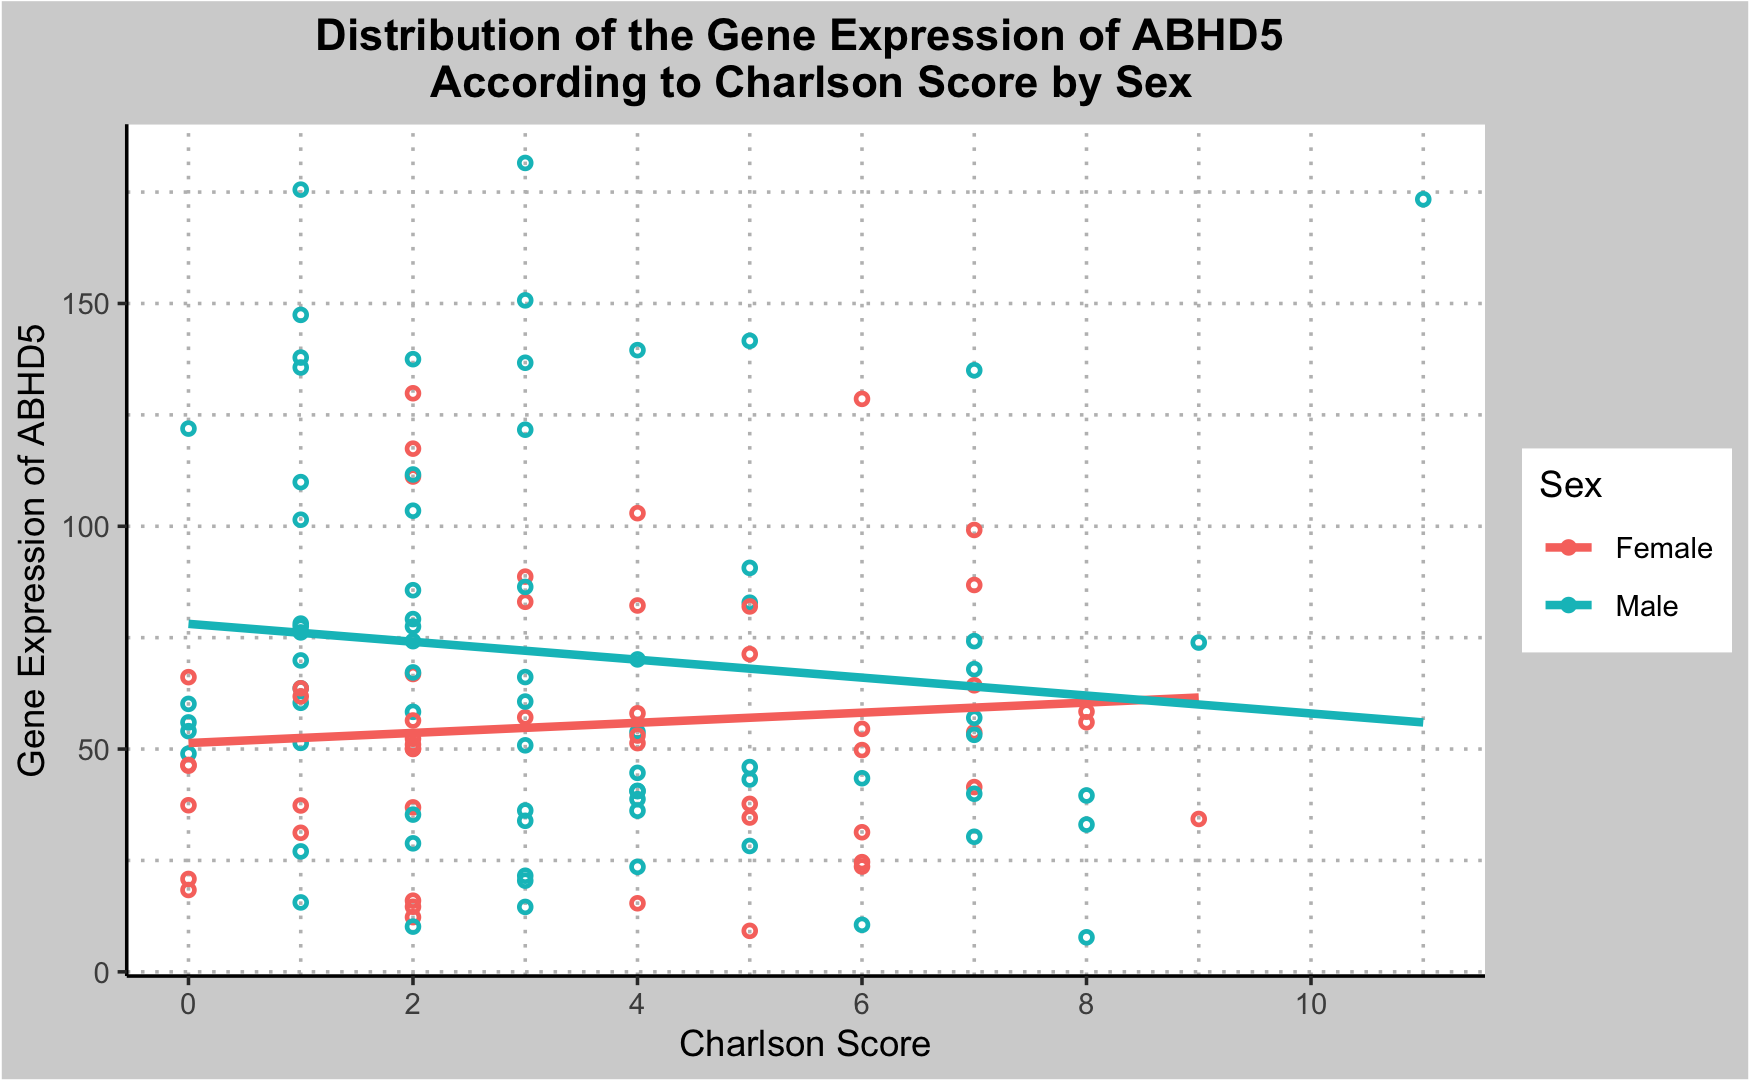
\includegraphics[width=1\linewidth]{Scatterplot.png}
    \label{fig:placeholder}
\end{figure}

Figure 2 is the scatterplot that shows the distribution of ABHD5 according to Charlson Score by sex. There appear to be distinct patterns between females and males in the relationship between ABHD5 expression and Charlson Score. In females, ABHD5 expression tends to increase as the Charlson Score increases, whereas in males, expression tends to decrease with higher Charlson Scores. Notably, the line graphs for both sexes converge at a Charlson Score of 9. However, given the presence of a significant outlier in the male group, this observed pattern requires further investigation to confirm its validity.

\subsection{Figure 3. Boxplot}
\begin{figure}[H]
    \centering
    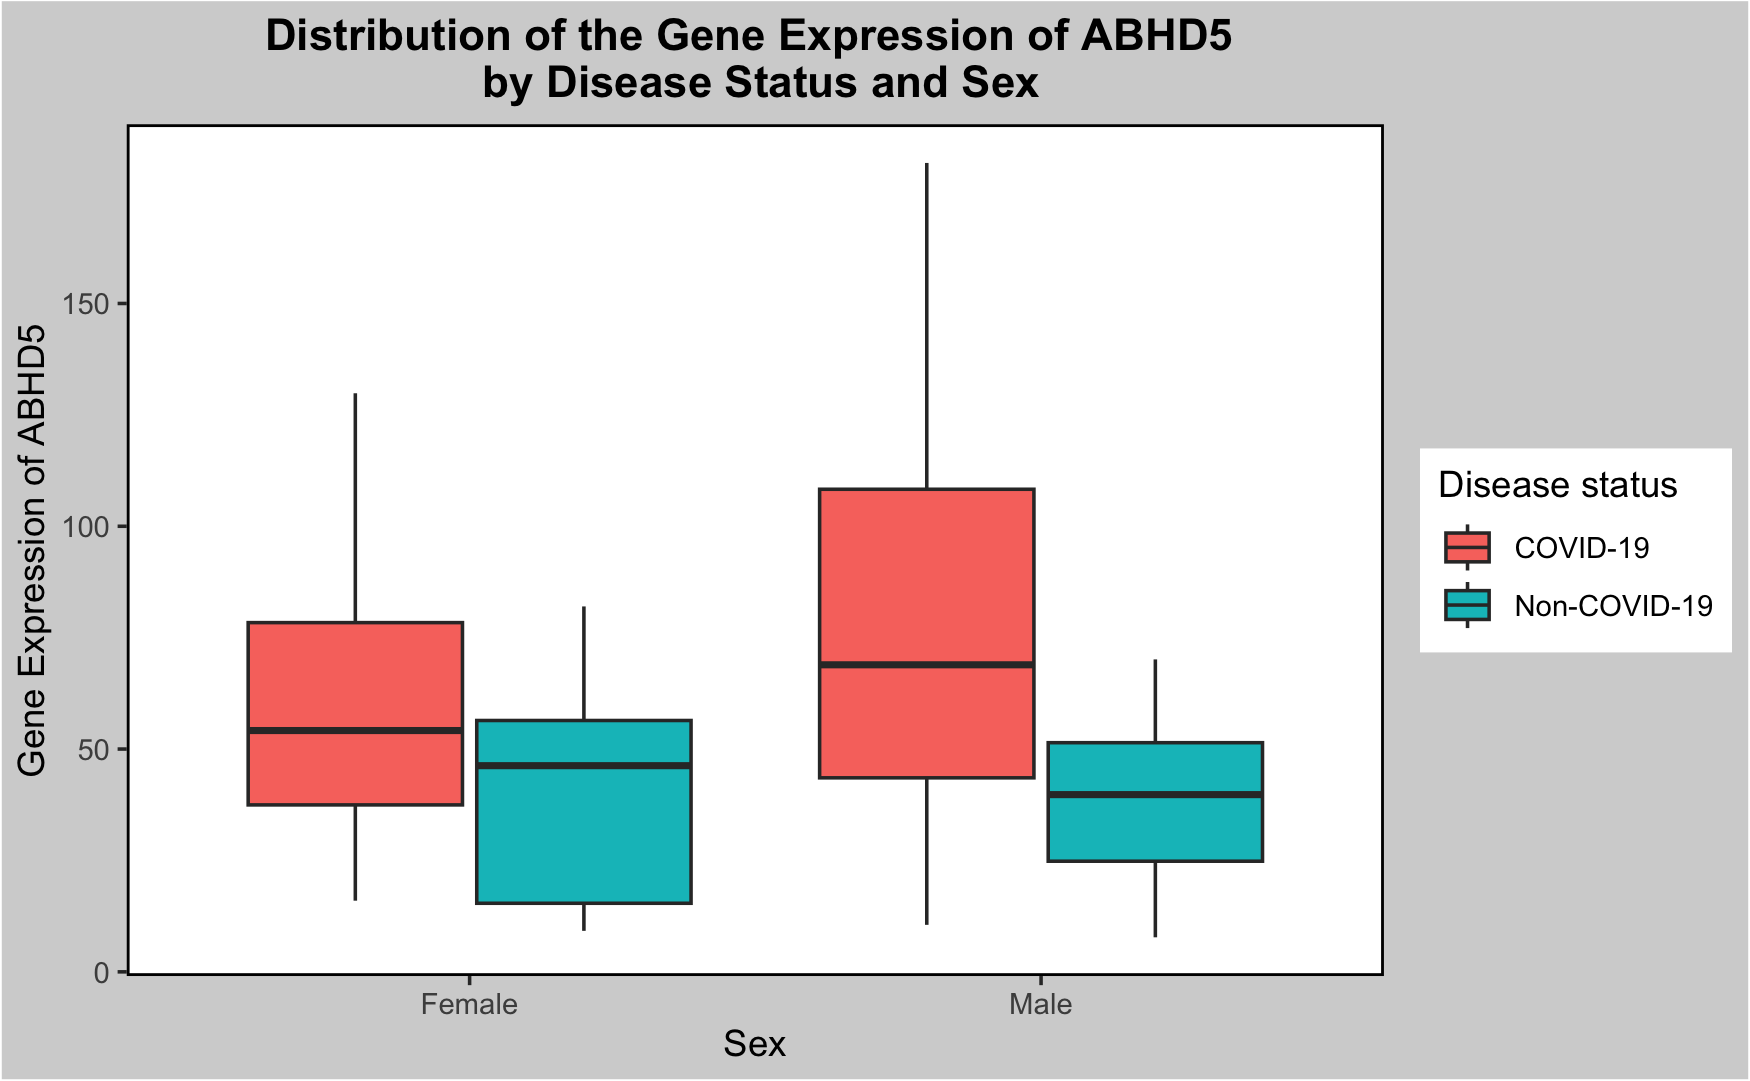
\includegraphics[width=1\linewidth]{Boxplot.png}
    \label{fig:placeholder}
\end{figure}

Figure 3 presents a boxplot illustrating the distribution of ABHD5 expression stratified by COVID-19 status and sex. Participants with COVID-19 show a significantly higher expression of ABHD5 compared to those without COVID-19. This trend is consistent across both female and male groups.

\subsection{Figure 4. Heatmap}
\begin{figure}[H]
    \centering
    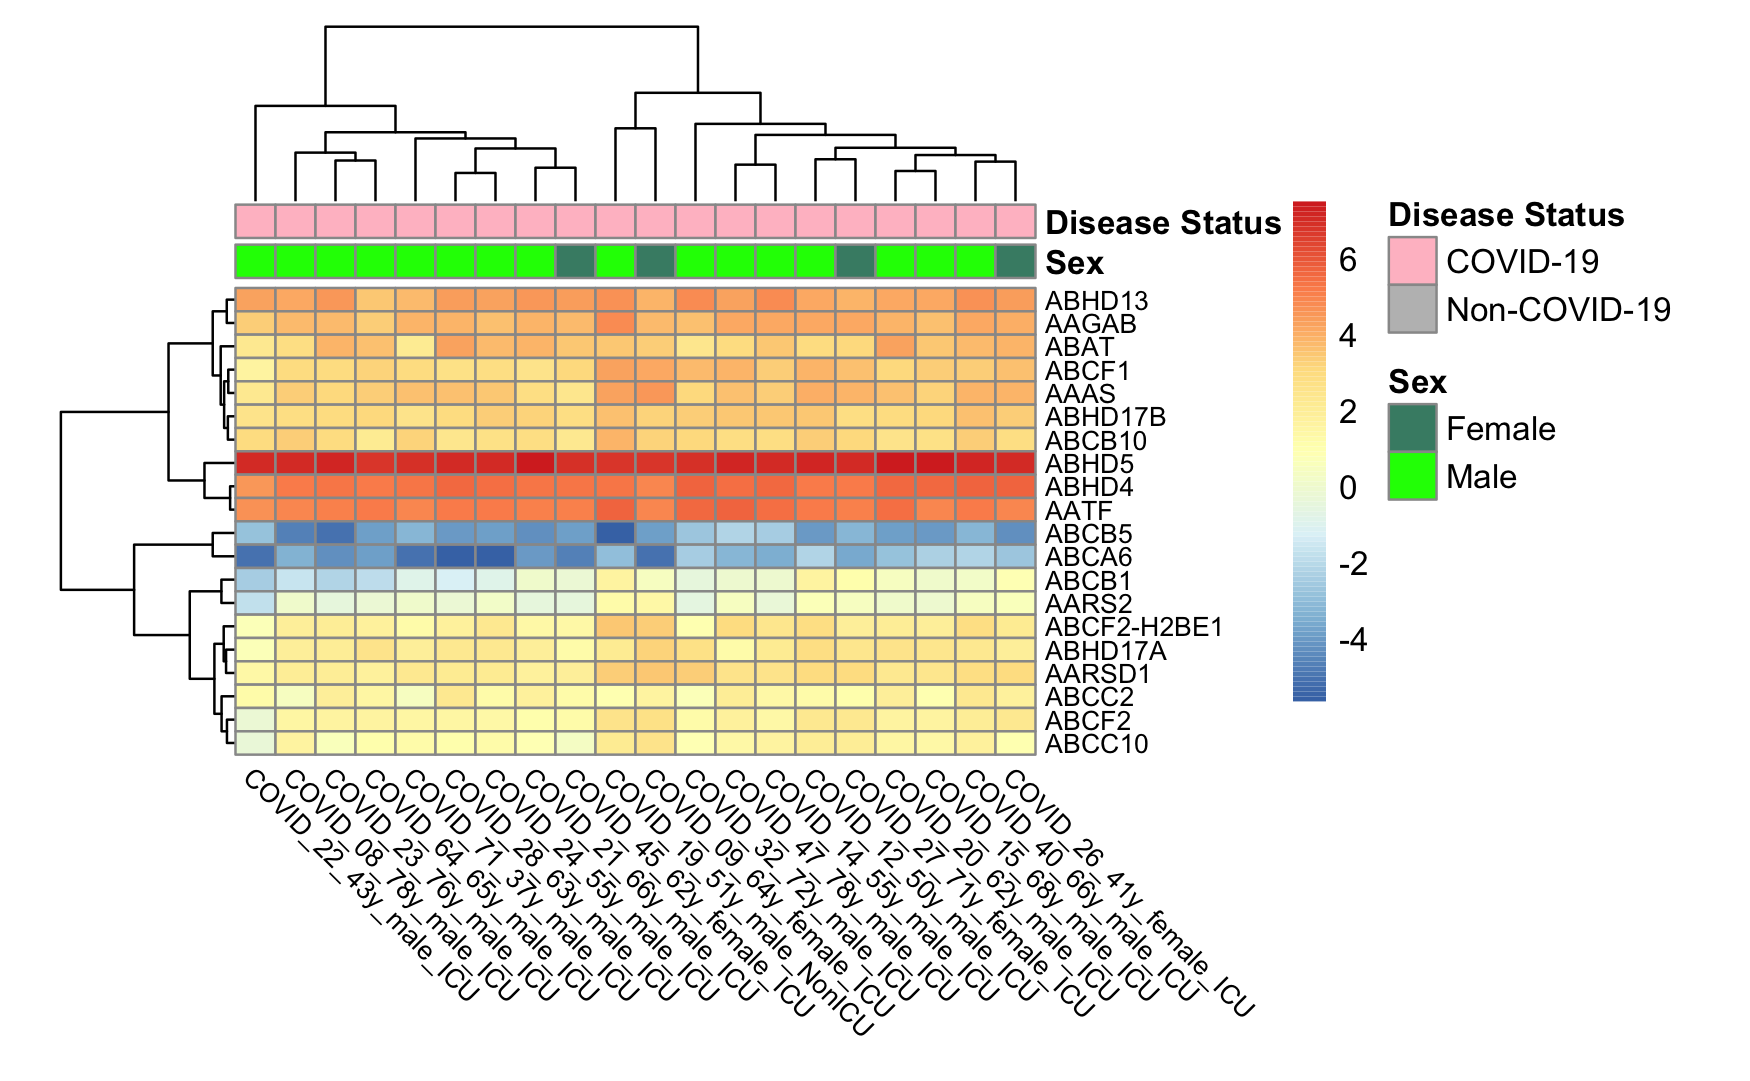
\includegraphics[width=1\linewidth]{Heatmap.png}
    \label{fig:placeholder}
\end{figure}

Figure 4 shows a heatmap illustrating the clustering of patients based on the top 20 genes with the highest expression variance, along with 19 additional randomly selected genes (including ABHD17A, ABCF2, ABCB5, ABCC2, ABCC10, ABHD4, ABCF1, ABHD17B, AATF, ABCB1, ABHD13, AAGAB, ABCA6, ABAT, ABCB10, AARSD1, AAAS, AARS2, and ABCF2-H2BE1), and ABHD5. Male participants and those with COVID-19 tend to exhibit greater variability in gene expression across these selected genes. However, since ABHD5 is generally highly expressed in humans and ABCA6 is known to have low expression, especially in non-relevant tissues, the interpretation of these particular genes within this clustering context may be limited or biologically insignificant.

\subsection{Figure 5. Hexbin}
\begin{figure}[H]
    \centering
    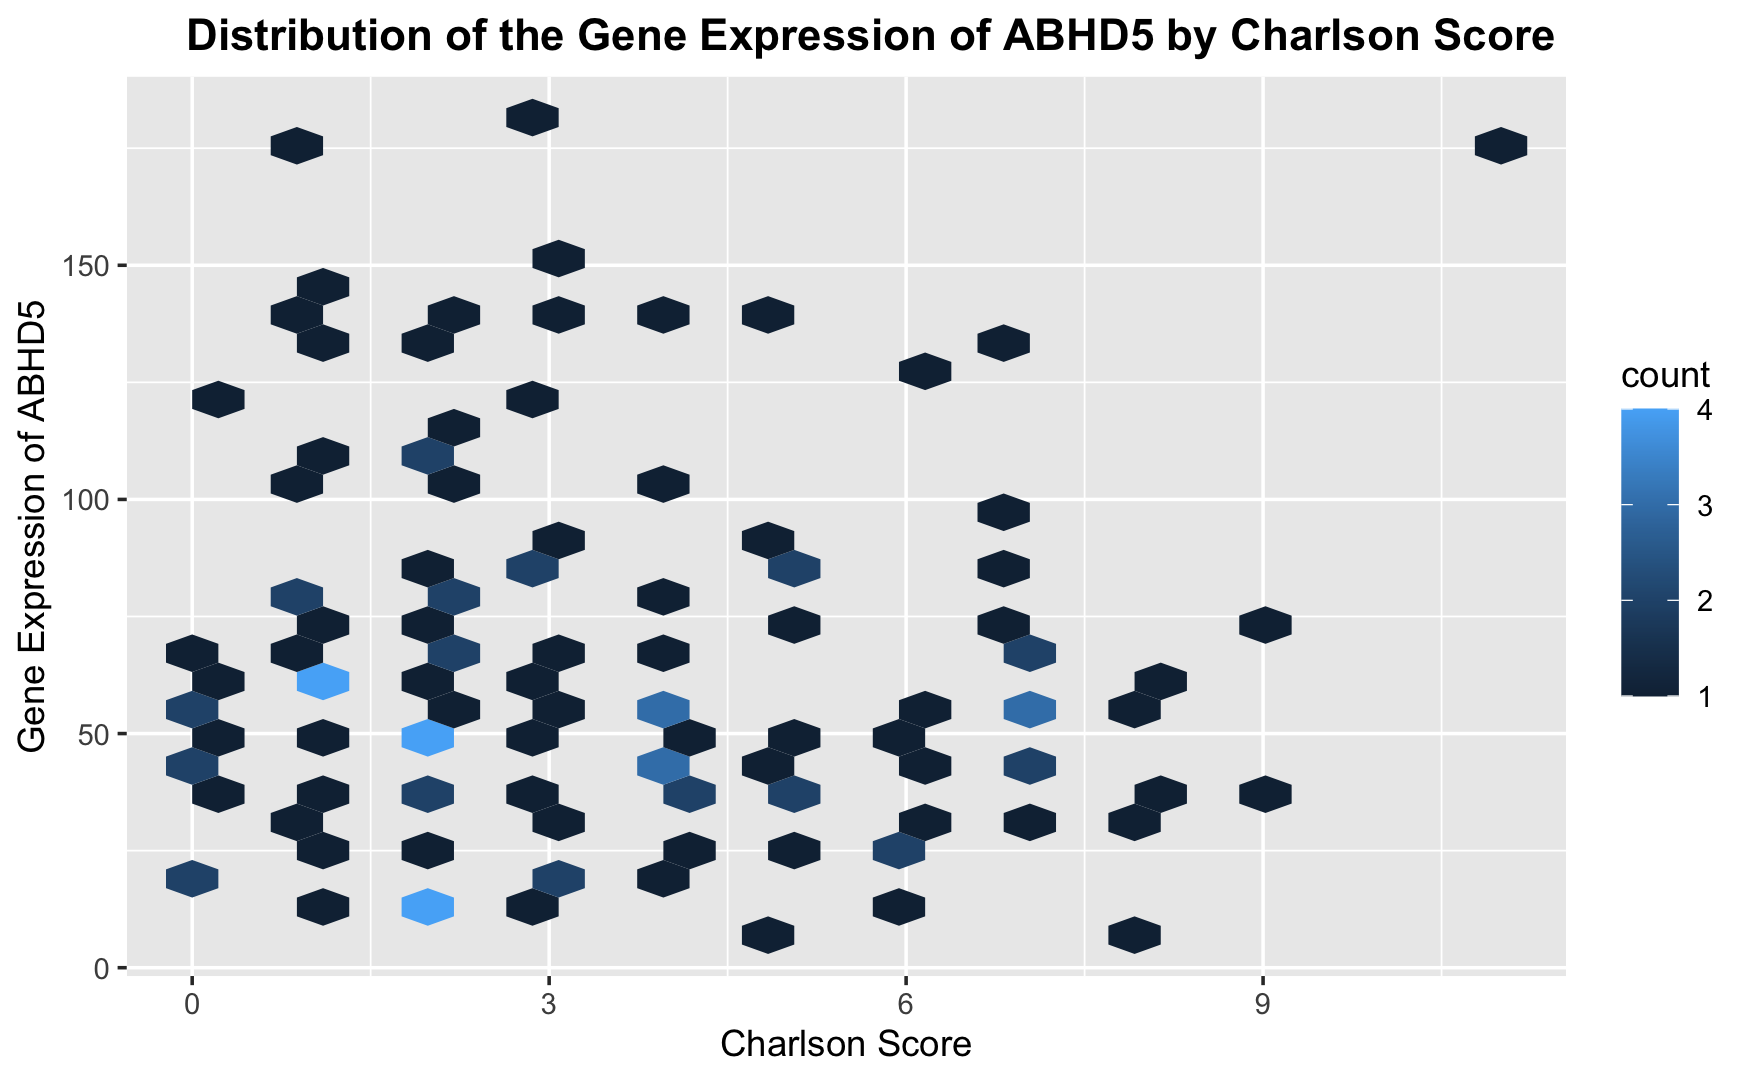
\includegraphics[width=1\linewidth]{Hexbin.png}
    \label{fig:placeholder}
\end{figure}

Compared to a scatterplot, the hexbin plot provides additional insights by visualizing point density and revealing distribution patterns that may be obscured by overplotting.

The distribution of ABHD5 gene expression appears to be highly variable across the full range of Charlson Scores. Most participants exhibit moderate expression levels (approximately 25–100), and no clear linear relationship is observed between Charlson Score and ABHD5 expression. Although a few high-expression outliers are present at higher Charlson Scores, suggesting potential areas for further investigation, the overall pattern indicates heterogeneous expression without a consistent trend.


\bibliographystyle{plain}
\clearpage
\begin{thebibliography}{9}

\bibitem{ref1}
ABHD5 abhydrolase domain containing 5 [Homo sapiens (human)] — Gene — NCBI.
\url{https://www.ncbi.nlm.nih.gov/gene/51099} . Accessed: 2025-08-21.

\bibitem{ref2}
Lass, A., Zimmermann, R., Haemmerle, G., Riederer, M., Schoiswohl, G., Schweiger, M., Kienesberger, P., Strauss, J. G., Gorkiewicz, G., \& Zechner, R. (2006). Adipose triglyceride lipase-mediated lipolysis of cellular fat stores is activated by CGI-58 and defective in Chanarin-Dorfman Syndrome. Cell metabolism, 3(5), 309–319. \url{https://doi.org/10.1016/j.cmet.2006.03.005}

\bibitem{ref3}
Schratter, M., Lass, A., \& Radner, F.P.W. (2022).
ABHD5—A regulator of lipid metabolism essential for diverse cellular functions.
Metabolites, 12(11), 1015. \url{https://doi.org/10.3390/metabo12111015}

\bibitem{ref4}
Gruber, A., Cornaciu, I., Lass, A., Schweiger, M., Poeschl, M., Eder, C., Kumari, M., Schoiswohl, G., Wolinski, H., Kohlwein, S. D., Zechner, R., Zimmermann, R., \& Oberer, M. (2010). The N-terminal region of comparative gene identification-58 (CGI-58) is important for lipid droplet binding and activation of adipose triglyceride lipase. The Journal of biological chemistry, 285(16), 12289–12298. 
\url{https://doi.org/10.1074/jbc.M109.064469}

\bibitem{ref5}
Overmyer, K. A., Shishkova, E., Miller, I. J., Balnis, J., Bernstein, M. N., Peters-Clarke, T. M., Meyer, J. G., Quan, Q., Muehlbauer, L. K., Trujillo, E. A., He, Y., Chopra, A., Chieng, H. C., Tiwari, A., Judson, M. A., Paulson, B., Brademan, D. R., Zhu, Y., Serrano, L. R., Linke, V., … Jaitovich, A. (2021). Large-Scale Multi-omic Analysis of COVID-19 Severity. Cell systems, 12(1), 23–40.e7. 
\url{https://doi.org/10.1016/j.cels.2020.10.003}

\bibitem{ref6}
Xie, Y. (2025). knitr: A General-Purpose Package for Dynamic Report Generation in R. R package version 1.50, \url{https://yihui.org/knitr/}

\bibitem{ref7}
Wickham, H., François, R., Henry, L., Müller, K. (2022). dplyr: A Grammar of Data Manipulation. \url{https://dplyr.tidyverse.org, https://github.com/tidyverse/dplyr.}

\bibitem{ref8}  
Zhu, H. (2024). kableExtra: Construct Complex Table with 'kable' and Pipe Syntax. 
\url {https://CRAN.R-project.org/package=kableExtra}

\bibitem{ref9}      
Rich, B. (2025). table1: Tables of Descriptive Statistics in HTML.
\url{https://github.com/benjaminrich/table1}

\bibitem{ref10} 
Wickham, H. (2016). ggplot2: Elegant Graphics for Data Analysis, Springer-Verlag New York.
\url{https://ggplot2.tidyverse.org}

\bibitem{ref11}  
Kolde, R. (2025). pheatmap: Pretty Heatmaps.
\url{https://CRAN.R-project.org/package=pheatmap}

\bibitem{ref12}
Carr, D., Lewin-Koh, N., Maechler, M., \& Sarkar, D. (2024). hexbin: Hexagonal Binning Routines.
\url {https://CRAN.R-project.org/package=hexbin}
\end{thebibliography}


\section*{Data and Code Availability}

The full analysis, code, figures, and report are publicly available on GitHub: \url{https://github.com/xiamy63/Final-project-MXIA}


\end{document}

